\documentclass[]{asme2ej}

%\usepackage{epsfig} %% for loading postscript figures
\usepackage{graphicx}
\graphicspath{ {images/} }

\usepackage{amsmath,amssymb}
\usepackage{hyperref}


\title{Exoplanet Direct Imaging Mission Simulation Code Interface Control Document}

%%% first author
\author{Daniel Garrett
    \affiliation{
	Graduate Research Assistant\\
	Cornell University\\
	Ithaca, NY 14850\\
    }	
}

%%% second author
\author{Dmitry Savransky
    \affiliation{ Professor\\
	Cornell University\\
	Ithaca, NY 14850
    }
}

\begin{document}

\maketitle    

%%%%%%%%%%%%%%%%%%%%%%%%%%%%%%%%%%%%%%%%%%%%%%%%%%%%%%%%%%%%%%%%%%%%%%
\begin{abstract}
{\it 
This document describes the required input/output interfaces between each stand-alone module in the exoplanet direct imaging mission simulation code.
}
\end{abstract}

\tableofcontents

%%%%%%%%%%%%%%%%%%%%%%%%%%%%%%%%%%%%%%%%%%%%%%%%%%%%%%%%%%%%%%%%%%%%%%
\begin{nomenclature}
\entry{HE}{Heliocentric Equatorial}
\entry{ICD}{Interface Control Document}
\entry{MJD}{Modified Julian Day}
\entry{OD}{Observatory Definition}
\entry{OSD}{Optical System Description}
\entry{PP}{Post-Processing}
\entry{PPD}{Planet Population Definition}
\entry{PPM}{Planet Physical Model}
\entry{SC}{Star Catalog}
\entry{SE}{Survey Ensemble}
\entry{SS}{Survey Simulation}
\entry{SU}{Simulated Universe}
\entry{TL}{Target List}
\end{nomenclature}

%%%%%%%%%%%%%%%%%%%%%%%%%%%%%%%%%%%%%%%%%%%%%%%%%%%%%%%%%%%%%%%%%%%%%%
% INTRODUCTION
%%%%%%%%%%%%%%%%%%%%%%%%%%%%%%%%%%%%%%%%%%%%%%%%%%%%%%%%%%%%%%%%%%%%%%

\section{Introduction}

The exoplanet direct imaging simulation code generates ensembles of mission simulations for exoplanet direct imaging missions to estimate science yields. The code consists of stand-alone modules written in Python which may be modified without requiring modifications to other portions of the code. This allows the code to be easily used to investigate new designs for exoplanet direct imaging missions. This document describes the required input/output interfaces for the stand-alone modules to enable this flexibility.

\subsection{Purpose}
This Interface Control Document (ICD) describes the interface between modules of the code. The data inputs and outputs of each module are described. Following these guidelines will allow the code to be updated to accommodate new mission designs.

\subsection{Scope}
This ICD defines the interfaces between modules of the code. It does not specify the contents of the individual modules beyond a general description of what each module does.

\subsection{Glossary}
This section will contain definition of terms used throughout the document if needed.

%%%%%%%%%%%%%%%%%%%%%%%%%%%%%%%%%%%%%%%%%%%%%%%%%%%%%%%%%%%%%%%%%%%%%%%%%%
% OVERVIEW
%%%%%%%%%%%%%%%%%%%%%%%%%%%%%%%%%%%%%%%%%%%%%%%%%%%%%%%%%%%%%%%%%%%%%%%%%%

\section{Overview}
The overall framework of the exoplanet direct imaging mission simulation code is depicted in Fig.~\ref{figure_framework}. The code framework consists of stand-alone modules. The fundamental inputs of the simulation may require external data. These include the Optical System Description (OSD), Star Catalog (SC), Planet Population Definition (PPD), Planet Physical Model (PPM), Observatory Definition (OD), Rules, and Post-Processing (PP) modules. The other modules used in mission simulation require a combination of the fundamental inputs as well as modules upstream in Fig.~\ref{figure_framework}. These include Target List (TL), Simulated Universe (SU), Survey Simulation (SS), and Survey Ensemble (SE) modules.

\begin{figure}[t]
    \centering
    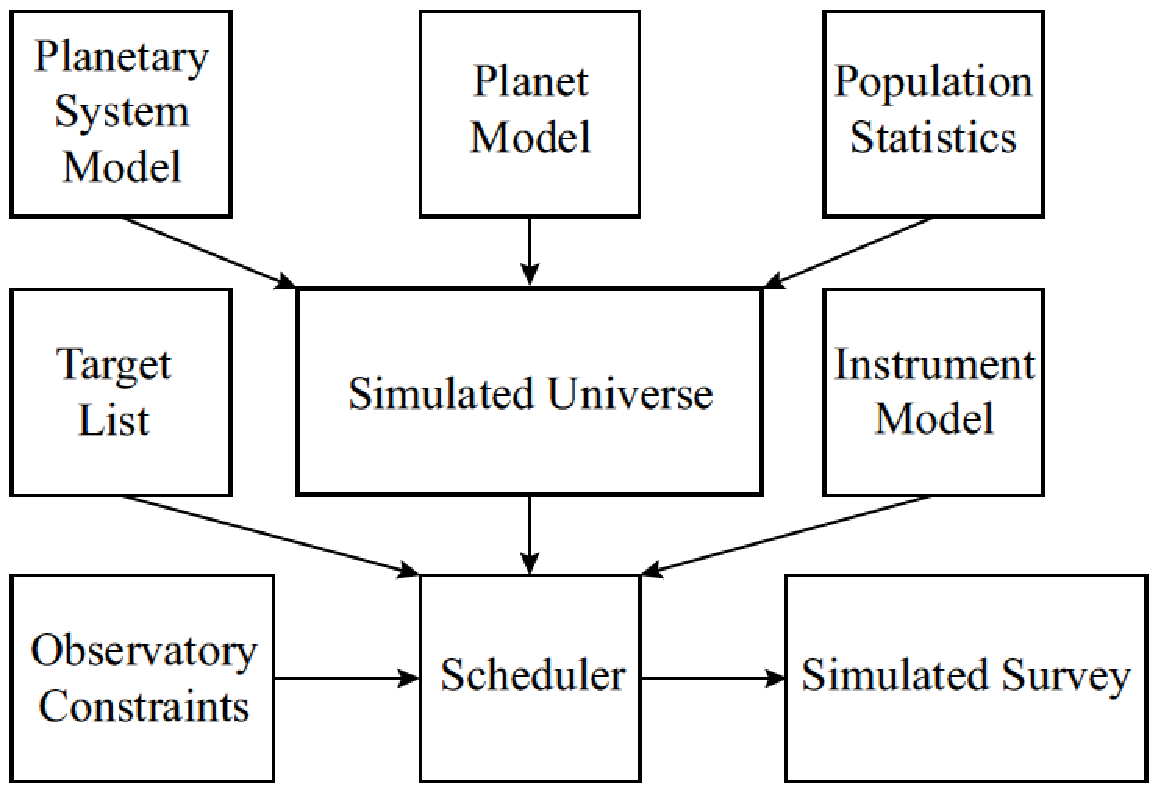
\includegraphics[width=5in]{Framework}
    \caption{Exoplanet direct imaging simulation code framework}
    \label{figure_framework}
\end{figure}

%%%%%%%%%%%%%%%%%%%%%%%%%%%%%%%%%%%%%%%%%%%%%%%%%%%%%%%%%%%%%%%%%%%%%%%%%
% GLOBAL SPECIFICATIONS
%%%%%%%%%%%%%%%%%%%%%%%%%%%%%%%%%%%%%%%%%%%%%%%%%%%%%%%%%%%%%%%%%%%%%%%%%

\section{Global Specifications}
This section specifies important information shared throughout the code.
\begin{description}
    \item[Common Epoch] \hfill \\ J2000
    \item[Common Reference Frame] \hfill \\ Heliocentric Equatorial (HE)
    \item[Common Time] \hfill \\ Modified Julian Day (MJD $\triangleq$ JD - 2400000.5)
\end{description}

\subsection{Python Packages}
The following Python packages are used for the WFIRST-specific version of exoplanet mission simulation:

\begin{itemize}
    \item astropy
        \begin{itemize}
            \item astropy.time
            \item astropy.units
        \end{itemize}
    \item numpy 
\end{itemize}

%%%%%%%%%%%%%%%%%%%%%%%%%%%%%%%%%%%%%%%%%%%%%%%%%%%%%%%%%%%%%%%%%%%%
% BACKBONE
%%%%%%%%%%%%%%%%%%%%%%%%%%%%%%%%%%%%%%%%%%%%%%%%%%%%%%%%%%%%%%%%%%%%

\section{Backbone}
All simulation execution will be performed by the backbone.  This set of functions will have very limited built-in functionality, and will primarily be tasked with parsing the input specification described below, and then calling the specified instances of each of the framework modules, detailed in \S\ref{sec:modules}.

A simulation specification is a single JSON-formatted (\url{http://json.org/}) file that encodes user-settable parameters and module names.  The backbone will contain a reference specification with \emph{all} parameters and modules set.  In the initial parsing of the user-supplied specification, it will be merged with the reference specification such that any fields not set by the user will be assigned to their reference (default) values. 

The backbone will contain a standalone specification parser that will check specification files for internal consistency.  For example, if modules carry mutual dependencies, the specification parser will return an error if these are not met for a given specification.  Similarly, if modules are selected with optional top level inputs, warnings will be generated if these are not set in the same specification files.

The backbone will contain an interactive function to help users generate specification files via a series of questions.

\subsection{Specification Format}
\begin{verbatim}
{
  "missionLifetime": 6,
  "missionDutyCycle": 0.24,
  "starlightSupressionSystems": [
    {
      "type": "SDO",
      "occulterDiameter": 50,
      "occulterDistance": 50000,
      "PSFfile": "/data/sdo1_psf.fits",
      "throughputFile": "/data/sdo1_thru.fits"
    },
    {
      "type": "coronagraph",
      "IWA": 3,
      "PSFfile": "/data/coron1_psf.fits",
      "throughputFile": "/data/coron1_thru.fits"
    }
  ],
  OSDmod: "hybridOSD1"
}
\end{verbatim}

%%%%%%%%%%%%%%%%%%%%%%%%%%%%%%%%%%%%%%%%%%%%%%%%%%%%%%%%%%%%%%%%%%%%%%%%%
% FUNDAMENTAL INPUT MODULE DESCRIPTION
%%%%%%%%%%%%%%%%%%%%%%%%%%%%%%%%%%%%%%%%%%%%%%%%%%%%%%%%%%%%%%%%%%%%%%%%%

\section{Modules of Fundamental Inputs}\label{sec:modules}
Modules containing fundamental inputs include Optical System Description (OSD), Star Catalog (SC), Planet Population Definition (PPD), Planet Physical Model (PPM), Observatory Definition (OD), Rules, and Post-Processing (PP). Much of the work of these modules will be reading external data and formatting the data for use by other modules. This section defines the input, output, and interface of each of these modules.

% OPTICAL SYSTEM DESCRIPTION NEEDS UPDATING

\subsection{Optical System Description (OSD) NEEDS UPDATING}
This module takes information about the optical system and formats the data into the specified outputs.

% STAR CATALOG

\subsection{Star Catalog (SC)}
This module takes information from a star catalog, such as Hipparcos, and formats the data into the specified outputs.

\subsubsection{Inputs}
\begin{description}
    \item[star catalog information] \hfill \\
    Information from an external star catalog containing the target stars
\end{description}

\subsubsection{Outputs} \label{starcatalog}
\begin{description}
    \item[missionsim.starcatalog.radeg] \hfill \\
    List of target star right ascension values in degrees
    \item[missionsim.starcatalog.decdeg] \hfill \\
    List of target star declination values in degrees
    \item[missionsim.starcatalog.pmra] \hfill \\
    List of target star right ascension proper motion values in mas/yr
    \item[missionsim.starcatalog.pmdec] \hfill \\
    List of target star declination proper motion values in mas/yr
    \item[missionsim.starcatalog.rv] \hfill \\
    List of target star radial velocities in km/s
    \item[missionsim.starcatalog.parx] \hfill \\
    List of target star parallax values in mas
\end{description}

% PLANET POPULATION DEFINITION NEEDS UPDATING

\subsection{Planet Population Definition (PPD) NEEDS UPDATING}
This module generates statistical distributions for planetary parameters.

% PLANET PHYSICAL MODEL NEEDS UPDATING

\subsection{Planet Physical Model (PPM) NEEDS UPDATING}
This module generates the planet physical models needed for simulation. These include models for albedo, phase, and reflected and emitted light.

% TIME KEEPING WORK IN PROGRESS
\subsection{Time}
This module contains all variables and functions related to global mission time and time tracking. There are two main tasks: lifetime and current mission time update.

\subsubsection{Lifetime}

\subsubsection*{Inputs}
\begin{itemize}
    \item
    \begin{description}
        \item[start] \hfill \\
        Mission start time in MJD
        \item[finish] \hfill \\
        Mission end time in MJD
    \end{description}
\end{itemize}

\subsubsection*{Outputs}
\begin{itemize}
    \item
    \begin{description}
        \item[missionsim.time.start] \hfill \\
        Mission start time in MJD
        \item[missionsim.time.finish] \hfill \\
        Mission end time in MJD
    \end{description}
\end{itemize}

\subsubsection{Current Mission Time Update}

\subsubsection*{Inputs}
\begin{itemize}
    \item 
    \begin{description}
        \item[missionsim.time.currenttime] \hfill \\
        Current mission time in MJD (offset to zero at mission start)
        \item[Time Step] \hfill \\
        Time step in MJD to next mission time
    \end{description}
\end{itemize}

\subsubsection*{Outputs}
\begin{itemize}
    \item
    \begin{description}
        \item[missionsim.time.currenttime] \hfill \\
        Update the mission time
    \end{description}
\end{itemize}

% OBSERVATORY DEFINITION CURRENTLY WORKING

\subsection{Observatory Definition (OD) CURRENTLY WORKING}
This module consists of three broad tasks: orbit, duty cycle, and keepout definition. The main inputs come externally and from the SC module.

\subsubsection{Orbit}

\subsubsection*{Inputs}
\begin{itemize}
    \item
    \begin{description}
        \item[Current Mission Time] \hfill \\
        Current mission time in MJD
    \end{description}
\end{itemize}

\subsubsection*{Outputs}
\begin{itemize}
    \item
    \begin{description}
        \item[missionsim.observatory.r\_sc] \hfill \\
        Observatory orbit position in HE reference frame at current mission time
    \end{description}
\end{itemize}

\subsubsection{Duty Cycle}

\subsubsection*{Inputs}
\begin{itemize}
    \item
    \begin{description}
        \item[Current Mission Time] \hfill \\
        Current mission time in MJD
    \end{description}
\end{itemize}

\subsubsection*{Outputs}
\begin{itemize}
    \item
    \begin{description}
        \item[missionsim.observatory.nexttime] \hfill \\
        Next available times in MJD
        \item[missionsim.observatory.nextduration] \hfill \\
        Time duration in MJD for next exoplanet detection and characterization referenced at \\ \texttt{missionsim.observatory.nexttime}
    \end{description}
\end{itemize}

\subsubsection{Keepout Definition}

\subsubsection*{Inputs}
\begin{itemize}
    \item
    \begin{description}
        \item[Current Mission Time] \hfill \\
        Current mission time in MJD 
        \item[missionsim.starcatalog] \hfill \\
        Output of SC module. See \ref{starcatalog} for definitions
    \end{description}
\end{itemize}

\subsubsection*{Outputs}
\begin{itemize}
    \item 
    \begin{description}
        \item[missionsim.observatory.ko] \hfill \\
        List of Boolean values for each target at current mission time where true is when a target is unobstructed in the keepout zone and false is when a target cannot be observed due to obstructions in the keepout zone
    \end{description}
\end{itemize}

% RULES NEEDS UPDATING

\subsection{Rules NEEDS UPDATING}
This module contains rules governing the simulation of exoplanet imaging missions.

% POST-PROCESSING NEEDS UPDATING

\subsection{Post-Processing (PP) NEEDS UPDATING}
This module describes the post-processing of results from the mission simulations.

%%%%%%%%%%%%%%%%%%%%%%%%%%%%%%%%%%%%%%%%%%%%%%%%%%%%%%%%%%%%%%%%%%%%%%%%%
% Modules using fundamental inputs
%%%%%%%%%%%%%%%%%%%%%%%%%%%%%%%%%%%%%%%%%%%%%%%%%%%%%%%%%%%%%%%%%%%%%%%%%

\section{Modules Using Internally Generated Data}
Modules using data generated by the fundamental input modules include Target List (TL), Simulated Universe (SU), Survey Simulation (SS), and Survey Ensemble (SE). These modules do not take any inputs external to the code.  They rely on information generated by other modules contained in the exoplanet mission simulation code.

% TARGET LIST NEEDS UPDATING

\subsection{Target List (TL) NEEDS UPDATING}
This module takes inputs from the OSD, SC, PPD, and OD modules to generate target list output.

% SIMULATED UNIVERSE NEEDS UPDATING

\subsection{Simulated Universe (SU) NEEDS UPDATING}
This module takes inputs from the TL and PPM modules to generate a simulated universe.

% SURVEY SIMULATION NEEDS UPDATING

\subsection{Survey Simulation (SS) NEEDS UPDATING}
This module takes inputs from the SU, PPD, Rules, OD, OSD, PP, and PPM modules to run a survey simulation.

% SURVEY ENSEMBLE NEEDS UPDATING

\subsection{Survey Ensemble (SE) NEEDS UPDATING}
This module takes inputs from the SS and PP modules to complete ensembles of mission simulations.

\end{document}
